\section{Python-Modul für Lineare und k-Nearest-Neighbor (KNN) Regression}


\subsection{
    Aufbau des Moduls \textit{V2A2\textunderscore Regression.py}
}

\subsubsection{ Klassen des Moduls \textit{V2A2\textunderscore Regression.py} und deren Zweck}

\subsubsection{ Zweck der Methoden \textit{fit(self,X,T),predict(self,x)} und \textit{crossvalidate(self,S,X,T)}}

\noindent
 \vspace{0px}
\textbf{fit(self,X,T):} Wird von abgeleiteten Klassen überschrieben. Berechnet die Regression mit Datenvektoren \textit{X} und Klassenlabels \textit{T}.

\noindent
 \vspace{0px}
\textbf{predict(self,x):} Wird von abgeleiteten Klassen überschrieben. Implementiert den Regressionsalgorithmus und berechnet den Zielvektor mit dem Datenvektor \textit{x}.

\noindent
 \vspace{0px}
\textbf{crossvalidate(self,S,X,T):} Führt die Kreuzvalidierung durch.


\subsubsection{ Unterschied  zwischen \textit{crossvalidate(.)} und der entsprechenden Methode für Klassifikation}

\noindent
 \vspace{0px}
Die Methode im vorherigen Versuch 1 hat die Wahrscheinlichkeit eines Klassifikationsfehlers und die Verwechslungsmatrix zurückgegeben, während die Methode in Versuch 2 Mittelwert, Standardabweichung, Maximum und Minimum des absoluten und relativen Fehlers zurückgibt. 

\subsection{
    Betrachtung der Funktion \textit{phi\textunderscore polynominal(x,deg)}
}

\subsubsection{ Berechnung und Ergebnis von \textit{phi\textunderscore polynominal(x,deg)} für verschiedene Werte}

Transformiert einen Datenvektor x in einen Merkmalsvektor \phi (x) mit dem Grad deg. 

\noindent
\textbf{phi\textunderscore polynomial([3],5):} liefert als Ergebnis den Merkmalsvektor [1, 3, 9, 27, 81, 243].
\noindent
\textbf{phi\textunderscore polynomial([3, 5],2):} liefert als Ergebnis den Merkmalsvektor [1, 3, 5, 9, 15, 25].

\subsubsection{ Allgemeine Formel für \textit{phi\textunderscore polynomial([x1,x2],2)} }

\begin{center}
    \phi (x) = [x\textsubscript{1,2}^0, x_1^1, x_2^1, x_1^2, x_1\cdot x_2, x_2^2]
\end{center}

\subsubsection{ Wozu braucht man diese Funktion im Zusammenhang mit Regression? }

\noindent
 \vspace{0px}
Man benötigt sie, um aus dem Vektor der Basisfunktionen die Designmatrix zu berechnen, mit welcher später die Normalgleichung aufgesytellt wird. 

\subsubsection{ Bis zu welchem Polynomgrad kann die Funktion Basisfunktionen berechnen? }

\noindent
 \vspace{0px}
Bis zum Grad 3.

\subsubsection{ Erweiterung bis zu Grad 5: }

\subsection{
    Betrachtung der Klasse \textit{LSRRegressifier}
}

\subsubsection{ Art des Regressionsmodells: }

\noindent
 \vspace{0px}
Der LSRRegressifier dient zum Minimieren der Least-Squares-Fehlerfunktion mit quadatischer Regulaisierung.

\subsubsection{ Parameter \textit{lmbda,phi,flagSTD} und \textit{eps} }

\noindent
 \vspace{0px}
\textbf{lambda:} Regularisierungskoeffizient. Gibt die relative Gewichtung zwischen dem Daten-Fehler und Gewichts-Fehler an. 
\noindent
 \vspace{0px}
\textbf{phi:} Vektor der Basisfunktionen aus dem die Designmatrix berechnet werden kann. 
\noindent
 \vspace{0px}
\textbf{flagSTD:} wird flagSTD>0 gewählt, werden die Daten auf einen Mittelwert = 0 und eine Standardabweichung = 1 skaliert.  
\noindent
 \vspace{0px}
\textbf{eps:} gibt die maximale Abweichung der Zielwerte von den prognostizierten Werten des linearen Modells an. 

\subsubsection{ Funktion der Klasse \textit{DataScaler}: }

\noindent
 \vspace{0px}
Die Klasse DataScaler standardisiert die Daten, wenn flagSTD>0 gesetzt ist. 
Data Scaler wird von der Klasse \textit{LSRRegressifier} in den Methoden \textit{fit(self,X,T,lmbda=None,phi=None,flagSTD=None)} und \textit{predict(self,x,flagSTD=None)} aufgerufen.


\subsubsection{ Wozu braucht man die Variablen \textit{Z} und \textit{maxZ} in der Methode \textit{fit(.)}? }

\noindent
 \vspace{0px}
Wenn das Problem gut konditioniert war, ergibt Variable \textit{Z} die Nullmatrix. \textit{maxZ} ist das größte Element der Matrix Z.
Wenn dieses kleiner ist als \textit{eps}, ist die gewünschte maximale Abweichung der Zielwerte von den prognostizierten Werten unterschritten. 

\subsubsection{ Vervollständigung der Methoden \textit{fit(self,X,T,...)} und \textit{predict(self,x,...)} }

\begin{figure}[H]
    \centering
    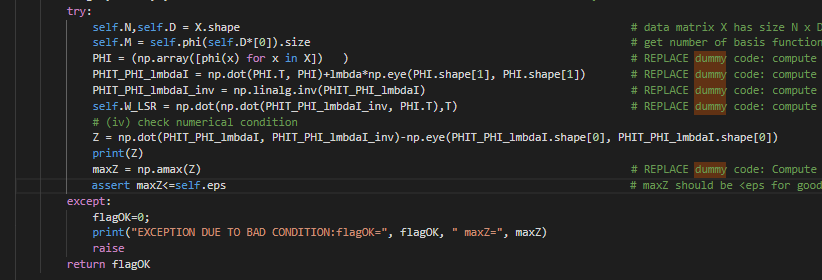
\includegraphics[width=1\linewidth]{aufgabe2c_fit.png}
\end{figure}

\subsection{
    Betrachtung der Klasse \textit{KNNRegressifier}
}

\subsubsection{ Art des Regressionsmodells: }

\noindent
 \vspace{0px}
K-Nearest-Neighbor Regression mit KD-trees. 

\subsubsection{ Parameter \textit{K} und \textit{flagKLinReg} }

\noindent
\textbf{Parameter K:} Anzahl der nächsten Nachbarn, die zur Berechnung der Wahrscheinlichkeit für die Klassenzugehörigkeit herangezogen werden.  

\noindent
\textbf{Parameter flagKLinReg:} Ist \textit{flagKLinReg}=0, wird einfach der Mittelwert der KNNs zurückgegeben.
Ansonsten wird die lineare Regression auf die KNNs angewendet. 

\subsubsection{ Berechnung der Prädiktion \textit{y(x_1)} }

\noindent
 \vspace{0px}
Die Methode \textit{predict(self,x,K=None,flagKLinReg=None)} holt sich zunächst die Indizes der K nächsten Nachbarn. 
Falls \textit{ flagKLinReg }=0 ist, wird mithilfe der Indizes einfach der Mittelwert der Klassenlabels T berechnet und zurückgegeben. 
Falls \textit{ flagKLinReg }>0 ist, wird die Klasse LSRRegressifier aufgerufen, welche zunächst mit \textit{ fit() } die Designmatrix, Gewichte, Abweichung der Zielwerte etc. berechnet und dann mit \textit{ predict() } die Zielwerte für den Textvektor x berechnet. 

\subsection{
    Betrachtung des Modultests
}

\subsubsection{ Beschreibung des Modultests: }

\subsubsection{ Welche Gewichte \textit{W} werden gelernt? Wie lautet die gelernte Prädiktionsfunktion? Welche Funktion sollte sich idealerweise für \textit{(N\rightarrow\infty)} ergeben? }

\subsubsection{ Ergebnisse der Kreuzvalidierung und Bedeutung der Werte }

\subsubsection{ Vergleich von Least Squares Regression und KNN-Regression }
